\chapter{Modelli di Fonti Luminose e Superfici}
\section{Modellazione di Superfici}
\begin{figure}[tb]
	\centering
	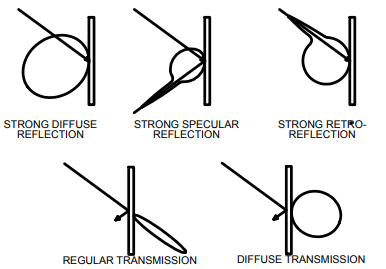
\includegraphics[width=0.4\linewidth]{../assets/chapter3_surfaces_interaction_types.png}
	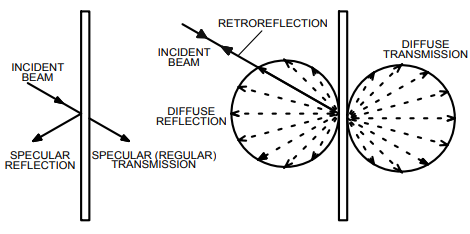
\includegraphics[width=0.4\linewidth]{../assets/chapter3_surfaces_specular_interaction.png}
	\label{chapter3:surface:interactionTypes}
	\caption{tipi di riflessione e trasmissione. Immagine da \cite{art-rad}}
\end{figure}
Quando un flusso radiante incide su una superficie, i tre processi che avvengono sono \textit{riflessione}, \textit{trasmissione}, 
\textit{assorbimento}, oltre all'emissione per tutti i materiali al di sopra dello zero assoluto. 
In particolare, durante la propagazione di un flusso radiante in un mezzo, parte della sua energia viene assorbita o 
deviata dal mezzo\footnote{d'ora in poi in questo capitolo si trascura la propagazione nel mezzo e si considera propagazione nel vuoto}.
Quando la luce incontra un oggetto, in particolare la sua superficie esterna, detta \textit{interfaccia}, tale flusso radiante pu\`o essere 
trasmesso e/o riflesso in diverse direzioni e con diversa intensit\`a.\par
Per il principio di conservazione dell'energia, all'interfaccia deve valere la propriet\`a\footnote{notazione introdotta in seguito}
\begin{equation}\label{chapter3:surface:interfaceEnergyConservation}
	\bar{\rho} + \bar{\uptau} = 1
\end{equation}
Si noti l'assenza del coefficiente di assorbimento, in quanto esso non \`e rilevante nell'interazione luce-interfaccia, ma partecipa in processi che 
coinvolgono la propagazione all'interno del volume del materiale, nel quale vale, per ogni lunghezza d'onda, in ogni istante, in ogni punto dello 
spazio, ancora la conservazione dell'energia
\begin{equation}\label{chapter3:surface:bulkEnergyConservation}
	\alpha + \rho + \uptau = 1
\end{equation}
Le propriet\`a ottiche che coinvolgono tali processi sono suddivise in spettrali e non, ed in estrinseche (suffisso "-ance") ed intrinseche 
(suffisso "-ivity"), queste ultime caratterizzanti il materiale ed utilizzate esclusivamente per materiali puri. In particolare seguono le definizioni
del CIE Lighting Vocabulary
\begin{altDescription}{chapter3:surface:coefficients}\label{chapter3:surface:coefficients}
	\item[\Gls{Reflectance}] \Glsdesc{Reflectance}. \mbox{Simbolo $\si{\rho}$}
	\item[\Gls{Transmittance}] \Glsdesc{Transmittance}. \mbox{Simbolo $\si{\uptau}$}
	\item[\Gls{Absorptance}] \Glsdesc{Absorptance}. \mbox{Simbolo $\si{\alpha}$}
	\item[\Gls{Reflectivity}] \Glsdesc{Reflectivity}. \mbox{Simbolo $\si{\rho_\infty}$}
	\item[\Gls{Transmissivity}] \Glsdesc{Transmissivity}. \mbox{Simbolo $\si{\uptau_u}$}
	\item[\Gls{Absorptivity}] \Glsdesc{Absorptivity}. \mbox{Simbolo $\si{\alpha_u}$}
\end{altDescription}
Si noti che nelle definizioni di Reflectivity e Transmissivity si contano anche i contributi aggiunti (nel primo caso) / tolti (nel secondo caso) per 
via del fenomeno di subsurface scattering\footnote{fuori scope}, dunque talvolta si considerano soltanto gli effetti di riflessione e trasmissione 
all'interfaccia, simboli $\bar{\rho}, \bar{\uptau}$, il cui valore per i vari materiali \`e governato dalle \textit{Equazioni di Fresnel} 
(vedi \ref{chapter3:surface:fresnel})
\begin{table}[tb!]
	\newcommand{\infint}[1]{\ensuremath{\int_0^\infty #1 \mathrm{d}\lambda}}
	\renewcommand\tabularxcolumn[1]{m{#1}}% for vertical centering text in X column
	\label{chapter3:surface:coefficientsFormulas}
	\begin{tabularx}{\linewidth}{cY}
		\toprule
		Coefficiente & Formula \\
		\midrule
		Spectral Reflectance & \[\rho_\lambda(\lambda)=\frac{\Phi_{e,\lambda}^r(\lambda)}{\Phi_{e,\lambda}^i(\lambda)}\] \\
		Reflectance & \[\rho = \frac{\Phi_e^r}{\Phi_e^i} = \frac{\infint{\rho_\lambda(\lambda)\Phi_{e,\lambda}^i}}{\infint{\Phi_{e,\lambda}^i}} %
							\neq \infint{\rho_\lambda(\lambda)}\]\\
		Spectral Transmittance & \[\rho_\lambda(\lambda)=\frac{\Phi_{e,\lambda}^r(\lambda)}{\Phi_{e,\lambda}^i(\lambda)}\] \\
		Trasmittance & \[\uptau = \frac{\Phi_e^t}{\Phi_e^i} = \frac{\infint{\uptau_\lambda(\lambda)\Phi_{e,\lambda}^i}}{\infint{\Phi_{e,\lambda}^i}} %
							\neq \infint{\uptau_\lambda(\lambda)}\]\\
		Spectral Absorptance & \[\alpha_\lambda(\lambda)=\frac{\Phi_{e,\lambda}^a(\lambda)}{\Phi_{e,\lambda}^i(\lambda)}\] \\
		Absorptance & \[\alpha = \frac{\Phi_e^a}{\Phi_e^i} = \frac{\infint{\rho_\lambda(\lambda)\Phi_{e,\lambda}^i}}{\infint{\Phi_{e,\lambda}^i}} %
							\neq \infint{\alpha_\lambda(\lambda)}\]\\
		\bottomrule
	\end{tabularx}
	\caption{formule per le definizioni \ref{chapter3:surface:coefficients}}
\end{table}
Nota dalla tabella \ref{chapter3:surface:coefficientsFormulas} come tali coefficienti dipendano dagli angoli solidi considerati per il calcolo del 
flusso incidente e riflesso/trasmesso. Distinguere tale computazione in categorie \`e pi\`u significativo per la reflectance 
(vedi \ref{chapter3:surface:nicodemusReflectances}).\par
Per caratterizzare macroscopicamente le propriet\`a di riflessione e trasmissione del materiale utilizziamo un approccio probabilistico, utilizzando 
una distribuzione\footnotemark{} che trasforma Irradianza incidente in Radianza riflessa o trasmessa. Nel caso della riflessione, non tutta la luce 
riflessa proviene dalla riflessione della luce incidente, ma pu\`o essere l'aggregato di contributi di riflessioni multiple in un materiale di spessore
finito, oppure radianza "riemersa" durante la propagazione all'interno del materiale per via di scattering multiplo. Nel caso di un materiale 
generico tale sarebbe eccessivamente dispendiosa. Nell'ipotesi che il materiale sia a regime, senza effetti di fosforescenza e 
fluorescenza (restringendoci all'ottica geometrica\footnotemark{}), possiamo modellare il materiale con una densit\`a di distribuzione che tiene conto 
della possibilit\`a di subsurface scattering nella superficie, approssimando il problema assumendo che la luce fuoriesca dal materiale soltanto in un 
punto, in un unica direzione. Tale densit\`a di distribuzione \`e detta \Gls{BSSRDF}(BSSRDF)
\begin{definitionS}
	La \Gls{BSSRDF}(BSSRDF) $S(\vec{p_o}, \hat{\omega_o}, \vec{p_i}, \hat{\omega_i})$ \Glsdesc{BSSRDF}
\end{definitionS}
\begin{equation}\label{chapter3:surface:bssrdf}
	S(\vec{p_o}, \hat{\omega_o}, \vec{p_i}, \hat{\omega_i}) = \frac{\mathrm{d}L_o(\vec{p_o},\hat{\omega_o})}{\mathrm{d}\Phi_i(\vec{p_i},\hat{\omega_i})}
\end{equation}
Approssimando ulteriormente il comportamento della luce, trascurando il fenomeno di subsurface scattering e supponendo che essa fuoriesca esclusiamente 
dal punto di incidenza (dunque soffermandoci soltanto sui fenomeni a livello dell'interfaccia), possiamo semplificare nella \Gls{BRDF}(BRDF)
\begin{definitionS}
	La \Gls{BRDF}(BRDF) $f_r(\vec{p},\hat{\omega_o},\hat{\omega_i})$ \Glsdesc{BRDF}
\end{definitionS}
\begin{equation}
	f_r(\vec{p},\hat{\omega_o},\hat{\omega_i}) = \frac{\mathrm{d}L_r(\vec{p}, \hat{\omega}_o)}{\mathrm{d}E_i(\vec{p}, \hat{\omega}_i)}
		= \frac{\mathrm{d}L_r(\vec{p}, \hat{\omega}_o)}{L_i(\vec{p}, \hat{\omega}_i)\langle\hat{n},\hat{\omega}_i\rangle\mathrm{d}\hat{\omega}_i}
\end{equation}
Le propriet\`a e casi d'uso di entrambe queste due distribuzioni saranno definite in seguito.\par
\footnotetext{Non propriamente una PDF, perch\`e non ha integrale unitario}
\footnotetext{In quanto le distribuzioni qui definite, nell'ipotesi di ottica geometrica, non cambiano la lunghezza d'onda della radiazione incidente, 
	la dipendenza di radianza, irradianza, flusso, con la lunghezza d'onda \`e omessa per comodit\`a}
Riconosciamo, a seconda della distribuzione spaziale della BRDF/BSSRDF, quattro tipologie di riflessione fondamentali, in particolare 
\begin{itemize}[topsep=0pt, noitemsep]
	\item[] \textit{Diffuse Reflection} la superficie si comporta come lambertiana rispetto alla riflessione, cio\`e distribuisce equamente 
		tutta\footnotemark{} il flusso incidente
	\item[] \textit{Glossy Specular Reflection} la superficie predilige un sottoinsieme di direzioni per la riflessione
	\item[] \textit{Perfectly Specular Reflection} la superficie riflette secondo la legge della riflessione per le superfici otticamente lisce
	\item[] \textit{Retroreflective Material} la superficie riflette gran parte del flusso nelle direzioni vicine a quella di incidenza
\end{itemize}
\footnotetext{Senza contare assorbimento}
Si noti che la trasmissione, modellata con una funzione analoga alla BRDF, la BTDF, \`e categorizzata in tre tipologie analoghe alle prime 
tre sopraindicate per la riflessione. Vedi figura \ref{chapter3:surface:interactionTypes}.\par
Come precedentemente accennato, per il calcolo della reflectance, vengono presi diversi angoli solidi come riferimento, vedi Tabella 
\ref{chapter3:surface:nicodemusReflectances}.
{
	\newcommand{\dotpr}[1]{\langle\hat{n},\hat{\omega}_{#1}\rangle}
	\newcommand{\iang}[2]{\int_{#1}f_r(\vec{p},\hat{\omega}_o,\hat{\omega}_i)\vert\dotpr{#2}\vert\mathrm{d}\hat{\omega}_{#2}}
	\renewcommand\tabularxcolumn[1]{m{#1}}% for vertical centering text in X column
	\begin{xltabular}{\linewidth}{YY}
		\caption{Tipi di reflectance proposti da \cite{nicodemus}. Nota che di solito il coseno dell'angolo rispetto allo zenith della direzione 
			incidente non \`e preso con valore assoluto, in quanto si assume $n$ come la normale che forma un angolo acuto con $\hat{\omega}_i$. 
			Seguendo la convenzione di \cite{pharr}, qui invece la normale \`e assunta sempre uscente dalla superficie.}
		\label{chapter3:surface:nicodemusReflectances}\\

		\toprule
		Coefficiente & Formula \\
		\midrule
		\endfirsthead

		\toprule
		\endhead

		\bottomrule
		\endfoot

		\bottomrule
		\endlastfoot

		Bidirectional Reflectance & \\
		\multicolumn{2}{>{\hsize=\dimexpr2\hsize- + 2\tabcolsep\relax}X}
			{\[\mathrm{d}\rho(\vec{p},\hat{\omega}_o, \hat{\omega}_i) = %
			f_r(\vec{p},\hat{\omega}_o,\hat{\omega}_i)\vert\dotpr{o}\vert\mathrm{d}\hat{\omega}_o\]} \\
		Directional-Conical Reflectance &\\
		\multicolumn{2}{>{\hsize=\dimexpr2\hsize- + 2\tabcolsep\relax}X}
			{\[\rho(\vec{p},\hat{\omega}_o,\hat{\omega}_i;\Omega) = \iang{\Omega}{o}\]}\\
		Directional-Hemispherical Reflectance &  \\
		\multicolumn{2}{>{\hsize=\dimexpr2\hsize- + 2\tabcolsep\relax}X}
			{\[\rho(\vec{p},\hat{\omega}_i) = \iang{\mathcal{H}^2(\hat{n})}{o}\]}\\
		Conical-Directional Reflectance &  \\
		\multicolumn{2}{>{\hsize=\dimexpr2\hsize- + 2\tabcolsep\relax}X}
			{\[\mathrm{d}\rho(\vec{p},\hat{\omega}_o,\hat{\omega}_i;\Omega) = %
			\frac{\vert\dotpr{o}\vert\mathrm{d}\hat{\omega}_o}{\int_{\mathcal{H}^2(\hat{n})}\vert\dotpr{i}\vert\mathrm{d}\hat{\omega}_i}
			\iang{\Omega}{i}\]}\\
		Biconical Reflectance &  \\
		\multicolumn{2}{>{\hsize=\dimexpr2\hsize- + 2\tabcolsep\relax}X}
			{\[\rho(\vec{p},\hat{\omega}_o,\hat{\omega}_i;\Omega_i,\Omega_o) =%
			\frac{1}{\int_{\mathcal{H}^2(\hat{n})}\vert\dotpr{i}\vert\mathrm{d}\hat{\omega}_i}%
			\int_{\Omega_i}\int_{\Omega_o}f_r(\vec{p},\hat{\omega}_o,\hat{\omega}_i)\vert\dotpr{o}%
			\dotpr{i}\vert\mathrm{d}\hat{\omega}_o\mathrm{d}\hat{\omega}_i\]}\\
		Conical-Hemispherical Reflectance &  \\
		\multicolumn{2}{>{\hsize=\dimexpr2\hsize- + 2\tabcolsep\relax}X}
			{\[\rho(\vec{p},\hat{\omega}_i;\Omega) =%
			\frac{1}{\int_{\mathcal{H}^2(\hat{n})}\vert\dotpr{i}\vert\mathrm{d}\hat{\omega}_i}%
			\int_\Omega\int_{\mathcal{H}^2(\hat{n})}f_r(\vec{p},\hat{\omega}_o,\hat{\omega}_i)\vert\dotpr{o}%
			\dotpr{i}\vert\mathrm{d}\hat{\omega}_o\mathrm{d}\hat{\omega}_i\]}\\
		Hemispherical-Directional Reflectance &  \\
		\multicolumn{2}{>{\hsize=\dimexpr2\hsize- + 2\tabcolsep\relax}X}
			{\[\mathrm{d}\rho(\vec{p},\hat{\omega}_o) =%
			\frac{\vert\dotpr{o}\vert\mathrm{d}\hat{\omega}_o}{\pi}\iang{\mathcal{H}^2(\hat{n})}{i}\]}\\
		Hemispherical-Directional Reflectance (alt)\footnotemark{} &  \\
		\multicolumn{2}{>{\hsize=\dimexpr2\hsize- + 2\tabcolsep\relax}X}
			{\begin{equation}\rho(\vec{p},\hat{\omega}_o) = \iang{\mathcal{H}^2(\hat{n})}{i}\end{equation}}\\
		Hemispherical-Conical Reflectance &  \\
		\multicolumn{2}{>{\hsize=\dimexpr2\hsize- + 2\tabcolsep\relax}X}
			{\[\rho(\vec{p}, \hat{\omega}_o;\Omega) = %
			\frac{1}{\pi}\int_{\mathcal{H}^2(\hat{n})}\int_\Omega f_r(\vec{p},\hat{\omega}_o,\hat{\omega}_i)\vert\dotpr{o}%
			\dotpr{i}\vert\mathrm{d}\hat{\omega}_o\mathrm{d}\hat{\omega}_i\]}\\
		Bi-Hemispherical Reflectance &  \\
		\multicolumn{2}{>{\hsize=\dimexpr2\hsize- + 2\tabcolsep\relax}X}
			{\begin{equation}\rho(\vec{p}) = \frac{1}{\pi}%
			\int_{\mathcal{H}^2(\hat{n}_i)}\int_{\mathcal{H}^2(\hat{n}_o)}f_r(\vec{p},\hat{\omega}_o,\hat{\omega}_i)\vert\dotpr{o}%
			\dotpr{i}\vert\mathrm{d}\hat{\omega}_o\mathrm{d}\hat{\omega}_i\end{equation}}\\
	\end{xltabular}
}
\footnotetext{La utilizziamo in seguito, per convenzione, senza normalizzazione e notazione differenziale. In tale contesto essa la chiamiamo "albedo"}
\subsection{Propriet\`a ottiche delle interfacce}\label{chapter3:surface:fresnel}
\begin{figure}[tb]
\colorlet{myblue}{blue!50!black!70}
\colorlet{glasscol}{blue!10}
\tikzstyle{glass}=[top color=glasscol!88!black,bottom color=glasscol,middle color=glasscol!98!black,shading angle=0]
\tikzset{
    light beam/.style={
        line width=1, 
        arrows={-Stealth[inset=1, angle=70:5]},
        draw=#1,
    },
    light beam/.default=myblue}
\newcommand\rightAngle[4]{
    \pgfmathanglebetweenpoints{\pgfpointanchor{#2}{center}}{\pgfpointanchor{#3}{center}}
    \coordinate (tmpRA) at ($(#2)+(\pgfmathresult+45:#4)$);
    \draw[white,line width=0.6] ($(#2)!(tmpRA)!(#1)$) -- (tmpRA) -- ($(#2)!(tmpRA)!(#3)$);
    \draw[blue!40!black] ($(#2)!(tmpRA)!(#1)$) -- (tmpRA) -- ($(#2)!(tmpRA)!(#3)$);
}
\centering
\begin{scaletikzpicturetowidth}{\linewidth}\begin{tikzpicture}[scale=\tikzscale]
    \def\L{6}   % width interface
    \def\l{1.5}   % length ray
    \def\t{1.3}   % depth glass gradient
    \def\h{1.3}   % bisector height
    \def\f{0.5}   % fraction of interface to the left
    \def\na{1.0}  % air
    \def\ng{1.5}  % glass
    \def\anga{65} % angle of incident ray
    \def\angg{asin(\na/\ng*sin(\anga))}
    \coordinate (O) at (0,0);            % point of contact
    \coordinate (I) at (90+\anga:\l);    % point incident (top left)
    \coordinate (M) at (90-\anga:\l);    % point reflected (top right)
    \coordinate (W) at (270-\anga:\l);   % opposite point reflected
    \coordinate (F) at ({-90+\angg}:\l); % point refracted (bottom)
    \coordinate (X) at (\l,0);           % x unit vector coordinate
    \coordinate (L) at (-\f*\L,0);       % left point interface
    \coordinate (R) at ({(1-\f)*\L},0);  % right point interface
    \coordinate (T) at (0,\h);           % top middle point (bisector)
    \coordinate (B) at (0,-1.0*\h);      % bottom middle point (bisector)
  
    % MEDIUM
    \fill[glass] (L) rectangle++ (\L,-\t); % glass gradient
    \fill[glasscol] (-\f*\L,-0.99*\t) rectangle ({1-\f)*\L},-\h); % glass bulk
    %\fill[glass] (L) rectangle (\L/2,-\h);
    \node[above=35, left=30] at (R) {$\eta_i$};
    \node[below=35, left=30] at (R) {$\eta_t>\eta_i$};
  
    % LINES
    \draw[light beam=black] (B) -- (T) node [black, below right=3] {$\hat{n}$}; % bisector
    \draw[light beam=black] (O) -- (X) node [black, above = 1.5] {$\hat{x}$}; % x unit vector
    \draw[light beam] (O) -- (I) node [black, left=1.5] {$\hat{\omega}_i$};
    \draw[light beam] (O) -- (M) node [black, right=1.5] {$\hat{\omega}_r$}; % reflected ray
    \draw[light beam=gray] (O) -- (W) node [left=1.5] {$-\hat{\omega}_r$};
    \draw[light beam] (O) -- (F) node [left=3] {$\hat{\omega}_t$}; % refracted ray

    % ORIGIN
    \draw[black,fill=white] (O) circle [radius=0.05] node [above right=0.5] {$\vec{p}$};
  
    % ANGLES
    \draw pic["$\theta_i$",draw=black,angle radius=40,angle eccentricity=1.3] {angle = T--O--I};
    \draw pic["$\theta_i$",draw=black,angle radius=40,angle eccentricity=1.3] {angle = W--O--B};
    \draw pic["$\theta_r$",draw=black,angle radius=40,angle eccentricity=1.3] {angle = M--O--T};
    \draw pic["$\theta_t$",draw=black,angle radius=40,angle eccentricity=1.3] {angle = B--O--F};
    \rightAngle{L}{O}{T}{0.3} 
\end{tikzpicture}\end{scaletikzpicturetowidth}
\caption{Illustrazione geometrica riflessione e rifrazione speculare}
\label{chapter3:surface:specular}
\end{figure}
Trascurando i fenomeni di scattering e assorbimento che avvengono all'interno del materiale, e concentrandoci solo sulle interazioni a livello di
interfaccia. Partiamo analizzando con queste convenzioni le superfici perfettamente speculari, la cui propagazione delle radiazioni, con assunzione di 
ottica geometrica, \`e interamente governata dalle 
\begin{align}\label{chapter3:surface:snell}
	\renewcommand{\arraystretch}{1.2}% like cases
	\setlength{\arraycolsep}{0pt}%
	\left.\begin{array}{ c r >{{}}l@{\quad} }
		\text{Legge della riflessione} & \theta_i &= \theta_r  \\
		\text{Legge di Snell\footnotemark{}} & \eta_i \sin\theta_i &= \eta_t\sin\theta_t \\
	\end{array}
	\right\}\varphi_o = \varphi_i + \pi
\end{align}
\footnotetext{Nota come i contributi delle varie lunghezze d'onda della radiazione incidente sono trasmessi ad angoli rispetto alla normale $\theta_t$ 
	differenti, effetto noto come \textit{Dispersione}. Ci\`o vuol dire che per ogni lunghezza d'onda campionata bisogna generare un nuovo raggio}
Ricordiamo che le implementazioni per la Legge di Snell devono tener conto della possibilit\`a di \textit{riflessione interna totale}, nel caso in
cui $\eta_t < \eta_i$ e \mbox{$\theta_i \geq \theta_c = \arcsin(\eta_i/\eta_t)$}.\par
Le direzioni di riflessione e rifrazione sono computate mediante osservazioni geometriche (Figura \ref{chapter3:surface:specular})
\begin{equation}
	\hat{\omega}_r = -(\hat{\omega}_i - 2\langle\hat{n},\hat{\omega}_i\rangle) = 2\langle\hat{n},\hat{\omega}_i\rangle - \hat{\omega}_i
\end{equation}
Mentre, per la trasmissione, sapendo che geometricamente 
\begin{equation}\label{chapter3:surface:directionComponents}
	\sin\theta_i\hat{x} = \cos\theta_i\hat{n} - \hat{\omega}_i
\end{equation}
e che per la legge di Snell
\begin{equation}\label{chapter3:surface:snellCosine}
	cos\theta_t = \sqrt{1-\sin^2\theta_t} = \sqrt{1-\frac{\eta_i^2}{\eta_t^2}\sin^2\theta_i} = \sqrt{1-\frac{\eta_i^2}{\eta_t^2}(1-\cos^2\theta_i)}
\end{equation}
allora la direzione di trasmissione
{
	\newcommand{\dotprr}{\langle\hat{n},\hat{\omega}_i\rangle}
	\newcommand{\eq}{\mathmakebox[\widthof{(\ref{chapter3:surface:snellCosine})}]{=}}
	\begin{align}
		\hat{\omega}_t \eq& \sin\theta_t\hat{x} - \cos\theta_t\hat{n} \\ 
			\stackrel{(\ref{chapter3:surface:directionComponents})}{\eq}&%
				\frac{\sin\theta_t}{\sin\theta_i}(\cos\theta_i\hat{n}-\hat{\omega}_i)-\cos\theta_t\hat{n} \nonumber \\
			\stackrel{(\ref{chapter3:surface:snell})}{\eq}&% 
				\left(\frac{\eta_i}{\eta_t}\cos\theta_i -\cos\theta_t\right)\hat{n}-\frac{\eta_i}{\eta_t}\hat{\omega}_i \nonumber \\
			\stackrel{(\ref{chapter3:surface:snellCosine})}{\eq}& \frac{\eta_i}{\eta_t}\left(\left(\cos\theta_i%
				-\frac{\eta_t}{\eta_i}\sqrt{1-\frac{\eta_i^2}{\eta_t^2}(1-\cos^2\theta_i)}\right)\hat{n}-\hat{\omega}_i\right)\nonumber \\
			\eq& \frac{\eta_i}{\eta_t}\left(\left(\cos\theta_i-\sqrt{\frac{\eta_t^2}{\eta_i^2}-1+\cos^2\theta_i)}\right)\hat{n}-\hat{\omega}_i\right)%
				\nonumber \\
			\eq& \frac{\eta_i}{\eta_t}\left(\left(\dotprr -\sqrt{\frac{\eta_t^2}{\eta_i^2}-1+\dotprr^2)}\right)\hat{n}-\hat{\omega}_i\right)
	\end{align}
}
Anche le frazioni di radiazione incidente trasmessa e riflessa dipendono dall'indice di rifrazione, secondo le \textit{Equazioni di Fresnel}, che 
forniscono le relazioni per il rapporto tra rispettivamente campo elettrico riflesso e campo elettrico incidente, e campo elettrico trasmesso 
e campo elettrico incidente, per ognuna delle due componenti di polarizzazione\footnotemark{}. Tali equazioni possono essere anche 
\footnotetext{\textit{polarizzazione s} (simbolo $\perp$), che indica che il campo elettrico oscilla con polarizzazione planare perpendicolarmente al 
	piano di incidenza, e \textit{polarizzazione p} (simbolo $\parallel$), che indica che il campo elettrico oscilla con polarizzazione planare 
	parallelamente al piano di incidenza}
espresse per relazionare i rapporti tra potenza riflessa e incidente, e potenza trasmessa e incidente\footnotemark{}.
\begin{align}
	\bar{\rho}_\perp(\mu) &= \frac{(a-\mu)^2+b^2}{(a+\mu)^2+b^2} \in [0,1] \\
	\bar{\rho}_\parallel(\mu) &= \frac{(a-\mu)^2+b^2}{(a+\mu)^2+b^2}\frac{(a-\frac{1-\mu^2}{\mu})^2+b^2}{(a-\frac{1+\mu^2}{\mu})^2+b^2} \in [0,1]\\
	\bar{\uptau}_\perp(\mu) &= \left(\frac{\eta_t}{\eta_i}\right)^2(1-\bar{\rho}_\perp) \\
	\bar{\uptau}_\parallel(\mu) &= \left(\frac{\eta_t}{\eta_i}\right)^2(1-\bar{\rho}_\parallel) \\
\end{align}
\footnotetext{Come prima detto, per la conservazione dell'energia, tali coefficienti devono sommarsi a 1, il che sembra essere in disaccordo con le 
	formule di trasmissione proposte. La motivazione risiede nel fatto che ci si sta riferendo a transmittance per radianze spettrali, per le quali 
	abbiamo citato si conserva la \textit{Radianza di base} (vedi \ref{chapter1:basicRadiance})}
dove
\begin{align*}
	\arraycolsep=1.4pt\def\arraystretch{2.2}
	\begin{array}{rlrl}
		a &= \sqrt{\displaystyle\frac{\sqrt{c^2+4\eta\kappa}+c}{2}} & \mu &= \cos\theta_i = \langle \hat{n},\hat{\omega}_i\rangle \\
		b &= \sqrt{\displaystyle\frac{\sqrt{c^2+4\eta\kappa}-c}{2}} & \mathclap{\eta\footnotemark{}} &= {\displaystyle\frac{\eta_i\eta_t+\kappa_t\kappa_i}{\eta_i^2+\kappa_i^2}} \\
		c &= \eta^2-\kappa^2-\left( 1-\mu^2\right) & \mathclap{\kappa\footnotemark{}} &= {\displaystyle\frac{\kappa_t\eta_i-\eta_t\kappa_i}{\eta_i^2+\kappa_i^2}}
	\end{array}
\end{align*}
\footnotetext{Indice relativo di rifrazione $\eta$ e indice relativo di asborption $\kappa$}
Per luce non polarizzata tali coefficienti sono pari alla media tra i coefficienti per polarizzazione-s e polarizzazione-p. Si mostra solo la formula 
per la riflessione.
\begin{equation}
	F_r(\mu) = \frac{\bar{\rho}_\perp(\mu)+\bar{\rho}_\parallel(\mu)}{2}
\end{equation}
